\documentclass[12pt]{article}
 \usepackage[margin=1in]{geometry} 
\usepackage{amsmath,amsthm,amssymb,amsfonts}
 \usepackage{graphicx}
\usepackage{caption}
\usepackage{subfigure}
\usepackage{pythonhighlight}

\newcommand{\N}{\mathbb{N}}
\newcommand{\Z}{\mathbb{Z}}
 
\newenvironment{problem}[2][Problem]{\begin{trivlist}
\item[\hskip \labelsep {\bfseries #1}\hskip \labelsep {\bfseries #2.}]}{\end{trivlist}}
%If you want to title your bold things something different just make another thing exactly like this but replace "problem" with the name of the thing you want, like theorem or lemma or whatever
 
\begin{document}
 
%\renewcommand{\qedsymbol}{\filledbox}
%Good resources for looking up how to do stuff:
%Binary operators: http://www.access2science.com/latex/Binary.html
%General help: http://en.wikibooks.org/wiki/LaTeX/Mathematics
%Or just google stuff
 
\title{Project 2B Report}
\author{Yutong Han 705025619 \\
		Yufeng Huang 704944399\\
		Yufei Hu 404944367\\
		Tianyi Liu 705035425 \\
		}
\maketitle
 
\section{Time Series Plot}

The Figure.\ref{fig:1} shows the time series plot( by day) of positive and negative sentiment.

\begin{figure}[!h]
     \begin{center}
                  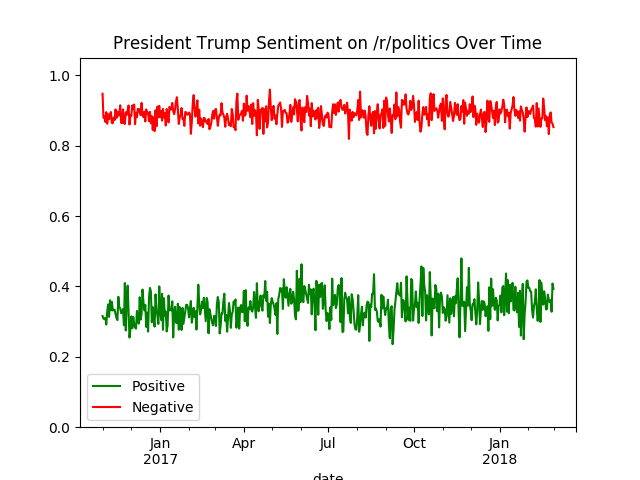
\includegraphics[width=0.8\textwidth]{../plots/part1.png}
    \end{center}
    \caption{%
       Time Series Plot 
     }%sl
   \label{fig:1}
\end{figure}



\section{Positive and Negative Sentiment of US State}

The Figure.\ref{fig:2} and Figure.\ref{fig:3} shows maps of the states of the United States for positive sentiment and one for negative sentiment.

\begin{figure}[!h]
      \centering
    \begin{subfigure}
        \centering
        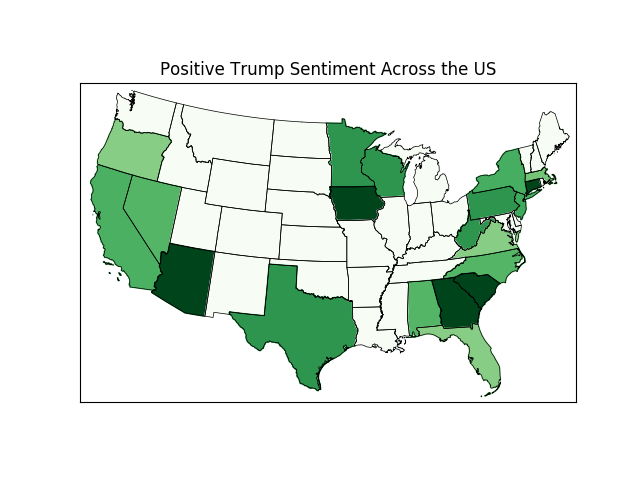
\includegraphics[width=0.7\textwidth]{../plots/part2_pos.png}
        \caption{Positive Sentiment over US States}
        \label{fig:2}
    \end{subfigure}%
    \vspace{1em}
    \begin{subfigure}
       \centering
        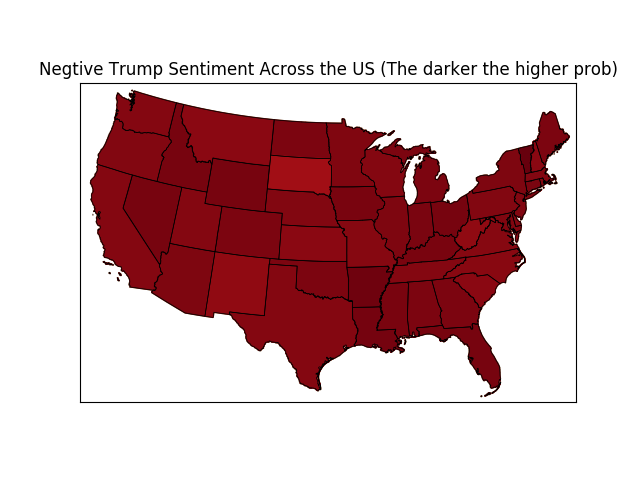
\includegraphics[width=0.7\textwidth]{../plots/part2_neg.png}
        \caption{Negative Sentiment over US States}
        \label{fig:3}
    \end{subfigure}
\end{figure}


\newpage 
\section{Sentiment Difference of US State}

The Figure.\ref{fig:4} shows the different of positive and negative sentiment across the US States.

\begin{figure}[!h]
     \begin{center}
                  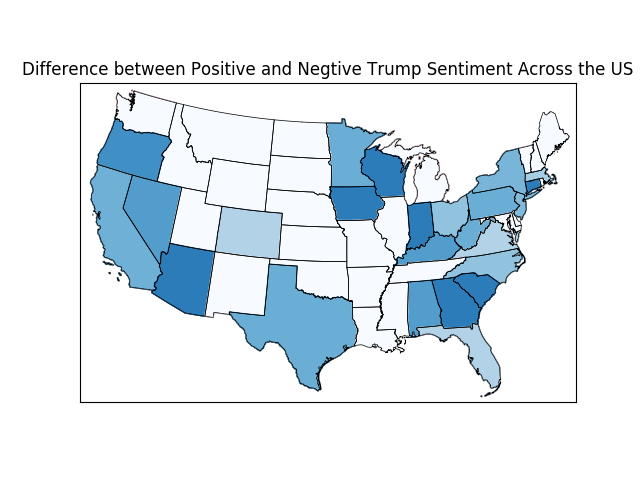
\includegraphics[width=0.8\textwidth]{../plots/part3.png}
    \end{center}
    \caption{%
       Difference between the positive and negative sentiment across US States.
     }%sl
     \label {fig:4}
 \end{figure}
 
\newpage  
\section{Top 10 positive stories}
 
The following two tables, table \ref{table1} and table \ref{table2} shows the list of top 10 positive stories and top 10 negative stories.\\
\begin{table}[!h]
\center
\caption{Top 10 positive stories}
\scalebox{0.9}{
\begin{tabular}{r|p{0.9\columnwidth}}
\hline
\textbf{ID} & \textbf{Title} \\\hline
dnzno4z & Diplomat regrets new turn with U.S \\\hline
dfs0vzl & Federal judge blocks Indiana abortion ultrasound mandate \\\hline
dop6avh & President Trump Promotes Book by Wonderful Pastor Who Says Satan Founded the Catholic Church\\\hline
dqsb8v2 & Prosecutors say longtime Manafort colleague has ties to Russian intelligence, the first such allegation by the special counsel\\\hline
dhsmsbd & Anderson Cooper to Trump surrogate: 'If he took a dump on his desk, you'd defend it' \\\hline
dht0d5u & WH Official: NYT, WaPo Reports Are 'Coordinated Attack' on Trump\\\hline
dryjzw2 & Russian tankers reportedly smuggling oil to North Korea: Trump has been silent, though one day earlier, he blasted China for the same thing.\\\hline
dkxzvnm & Ben Shapiro: 'Views Should Never be Banned'\\\hline
dlbi7zb & Feinstein: We Can't Increase Immigration Enforcement Because No One Will Pick Our Fruit \\\hline
dmtjwsg &  Mr. President, They're Never Going To Like You\\\hline
\end{tabular}}
\label{table1}
\end{table}


\begin{table}[!h]
\center
\caption{Top 10 negative stories}
\scalebox{0.9}{
\begin{tabular}{r|p{0.9\columnwidth}}
\hline
\textbf{ID} & \textbf{Title} \\\hline
dtl0kfs & FBI director prepared to issue rebuttal if Nunes memo released \\\hline
den7nsu & Adding a Dislike Button to Twitter Could Neutralize Trump's Social Media Presence\\\hline
di419p4 & 'This is off the map': Former intelligence officials say the reported Kushner-Russia plan is unlike anything they've ever seen\\\hline
dhnhxbt & Graham invites Comey to testify before Senate panel  \\\hline
diw3ehp & Rep. DeSantis: Man Asked Whether Republicans or Dems Were on Field Before Scalise Shooting\\\hline
dozvoc1 & Former President Obama called for jury duty in Chicago \\\hline
dg76w4g & Trump Says He May Freeze Subsidies to the Poor Until Democrats Repeal Obamacare\\\hline
dhc6yws & Republican Senator Graham to examine Trump's business deals: CNN\\\hline
di8wivz & GOP taps anti-Clinton strategy to damage Elizabeth Warren early \\\hline
dje8p0t & Russian Agents Used High Tech Alien Technology To Collude With Trump While Hiding Under James Comey's Floorboards, Sources Say \\\hline
\end{tabular}}
\label{table2}
\end{table}


\section{Scatterplots of Submission Score and Comment Score}

The Figure.\ref{fig:5} and Figure.\ref{fig:6} are the scatterplots where the X axis is the submission score, and a second where the X axis is the comment score, and the Y access is the percentage positive and negative. The two different colors for positive and negative.
\begin{figure}[!h]
      \centering
    \begin{subfigure}
        \centering
        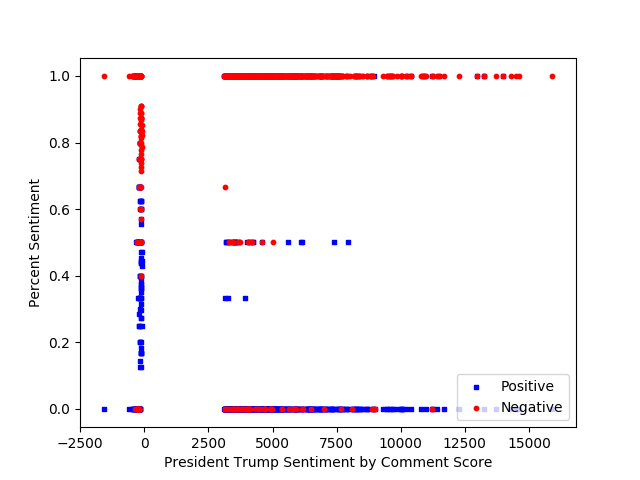
\includegraphics[width=0.65\textwidth]{../plots/part5_com.png}
        \caption{Sentiment by comment score}
        \label{fig:5}
    \end{subfigure}%
    \vspace{1em}
    \begin{subfigure}
       \centering
        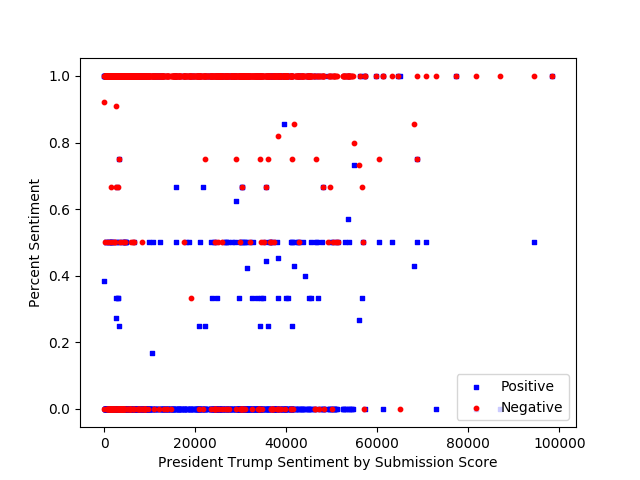
\includegraphics[width=0.65\textwidth]{../plots/part5_sub.png}
        \caption{Sentiment by submission score}
        \label{fig:6}
    \end{subfigure}
\end{figure}


\section{Producing the ROC curves}

The Figure.\ref{fig:7} plot the ROC for the classifier.
\begin{figure}[!h]
     \begin{center}
                  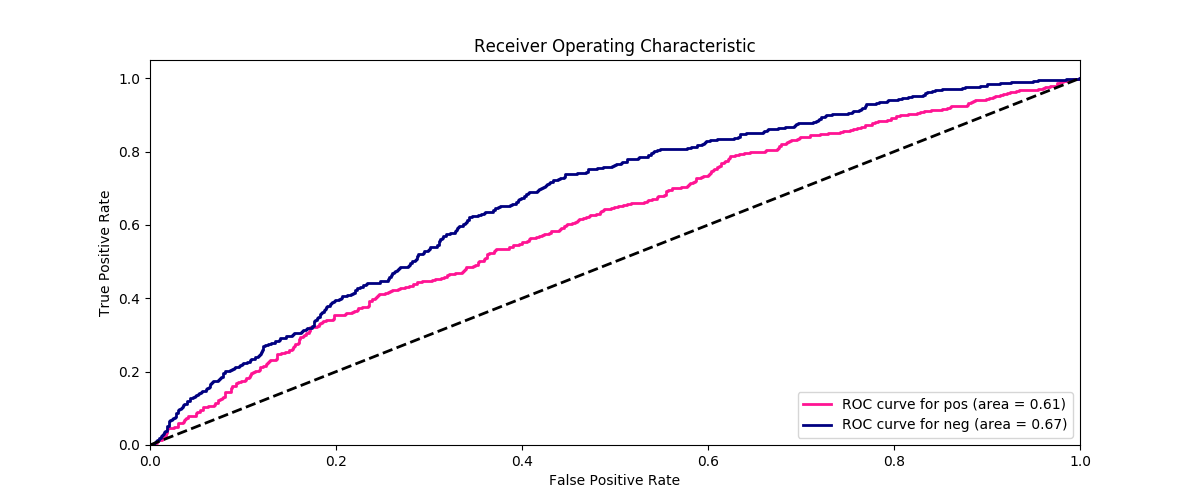
\includegraphics[width=0.8\textwidth]{../plots/part7.png}
    \end{center}
    \caption{%
       Receiver Operating Characteristic
     }%sl
   \label{fig:7}
\end{figure}

\section {Summarizing finding}

Through the change of the time curve, we can clearly see that Trump's positive comment has steadily and slightly increased with the increase of Trump's ruling time. However, on the whole, the fact that the majority of the comments about President Trump is negative did not change at all.

What's more, surprisingly, the distribution of positive and negative sentiment towards Trump across the US States is not based on the states that we envisioned to support Republicans or Democrats. In other words, there is no significant difference between the states.

What we do expect is that the comment's sentiment differs in different stories. People inclined to express their negative comment for the Trump Russia scandal, the performance of Trump in social media and some crazy and some his irresponsible speech. But when it comes to immigration and religion, people have more ratio of positive sentiment.

As far as I am concerned, all the mentioned phenomenon can be explained by an extremely important and essential question that who are the voters of Trump, which is also the reason why Trump won the election the president of America. According to plenty of sociology and political literature, the claim that white working-class voters were a crucial block of support for Trump in the 2016 presidential election has been the consensus in the academic. It is the silent majority that makes Trump become president and at the same time those people's opinion and sentiment toward Trump is very difficult to detect by political blog statistics or public opinion poll.
\newpage
\section {Question 1}

Take a look at $labeled\_data.csv$ Write the functional dependencies implied by the data.

\textbf {Answer:} The $Input\_id$ is the primary key of the scheme. So the $Input\_id \to labeldem$,  $Input\_id \to labelgop$, $Input\_id \to labeldjt$ and their combinations can be implied. 
\section {Question 2}
Take a look at the schema for the comments dataframe. Forget BCNF and 3NF. Does the data frame look normalized? In other words, is the data frame free of redundancies that might affect insert/update integrity? If not, how would we decompose it? Why do you believe the collector of the data stored it in this way?

\textbf{Answer:} It does not look normalized. In the $subreddit\_id$ and $subreddit$ part, it seems that the  $subreddit\_id \to subreddit$. So the $subreddit$ may store repeatedly. So it can be decomposed into two scheme with the $subreddit$ be the key of other scheme. Since this database may contains about the posts about the politics, the subreddit is just the \textit{/r/politics}


\section {Question 3}
Pick one of the joins that you executed for this project. Return the join with .explain() attached to it. Include the output. What do you notice? Explain what Spark SQL is doing during the join. Which join algorithm does Spark seem to be using?

\textbf{Answer:} The Figure.\ref{fig:explain} shows the output of the .explain on the join operation 
\begin{python}
df_full = df_com_full
	.join(df_sub_full, 
	df_com_full.link_id == df_sub_full.sub_id, 
	'inner')
\end{python}

Here we can notice that the Spark use the Hash Join algorithm (BroadcastHashJoin) and build the index on the right relation.  Spark first loads each relation and filter the not null key value we want to join on. Then project the values we want to select. And finally do the hash join on two relations using the Hash Join alogorithm.

\begin{figure}[!h]
     \begin{center}
                  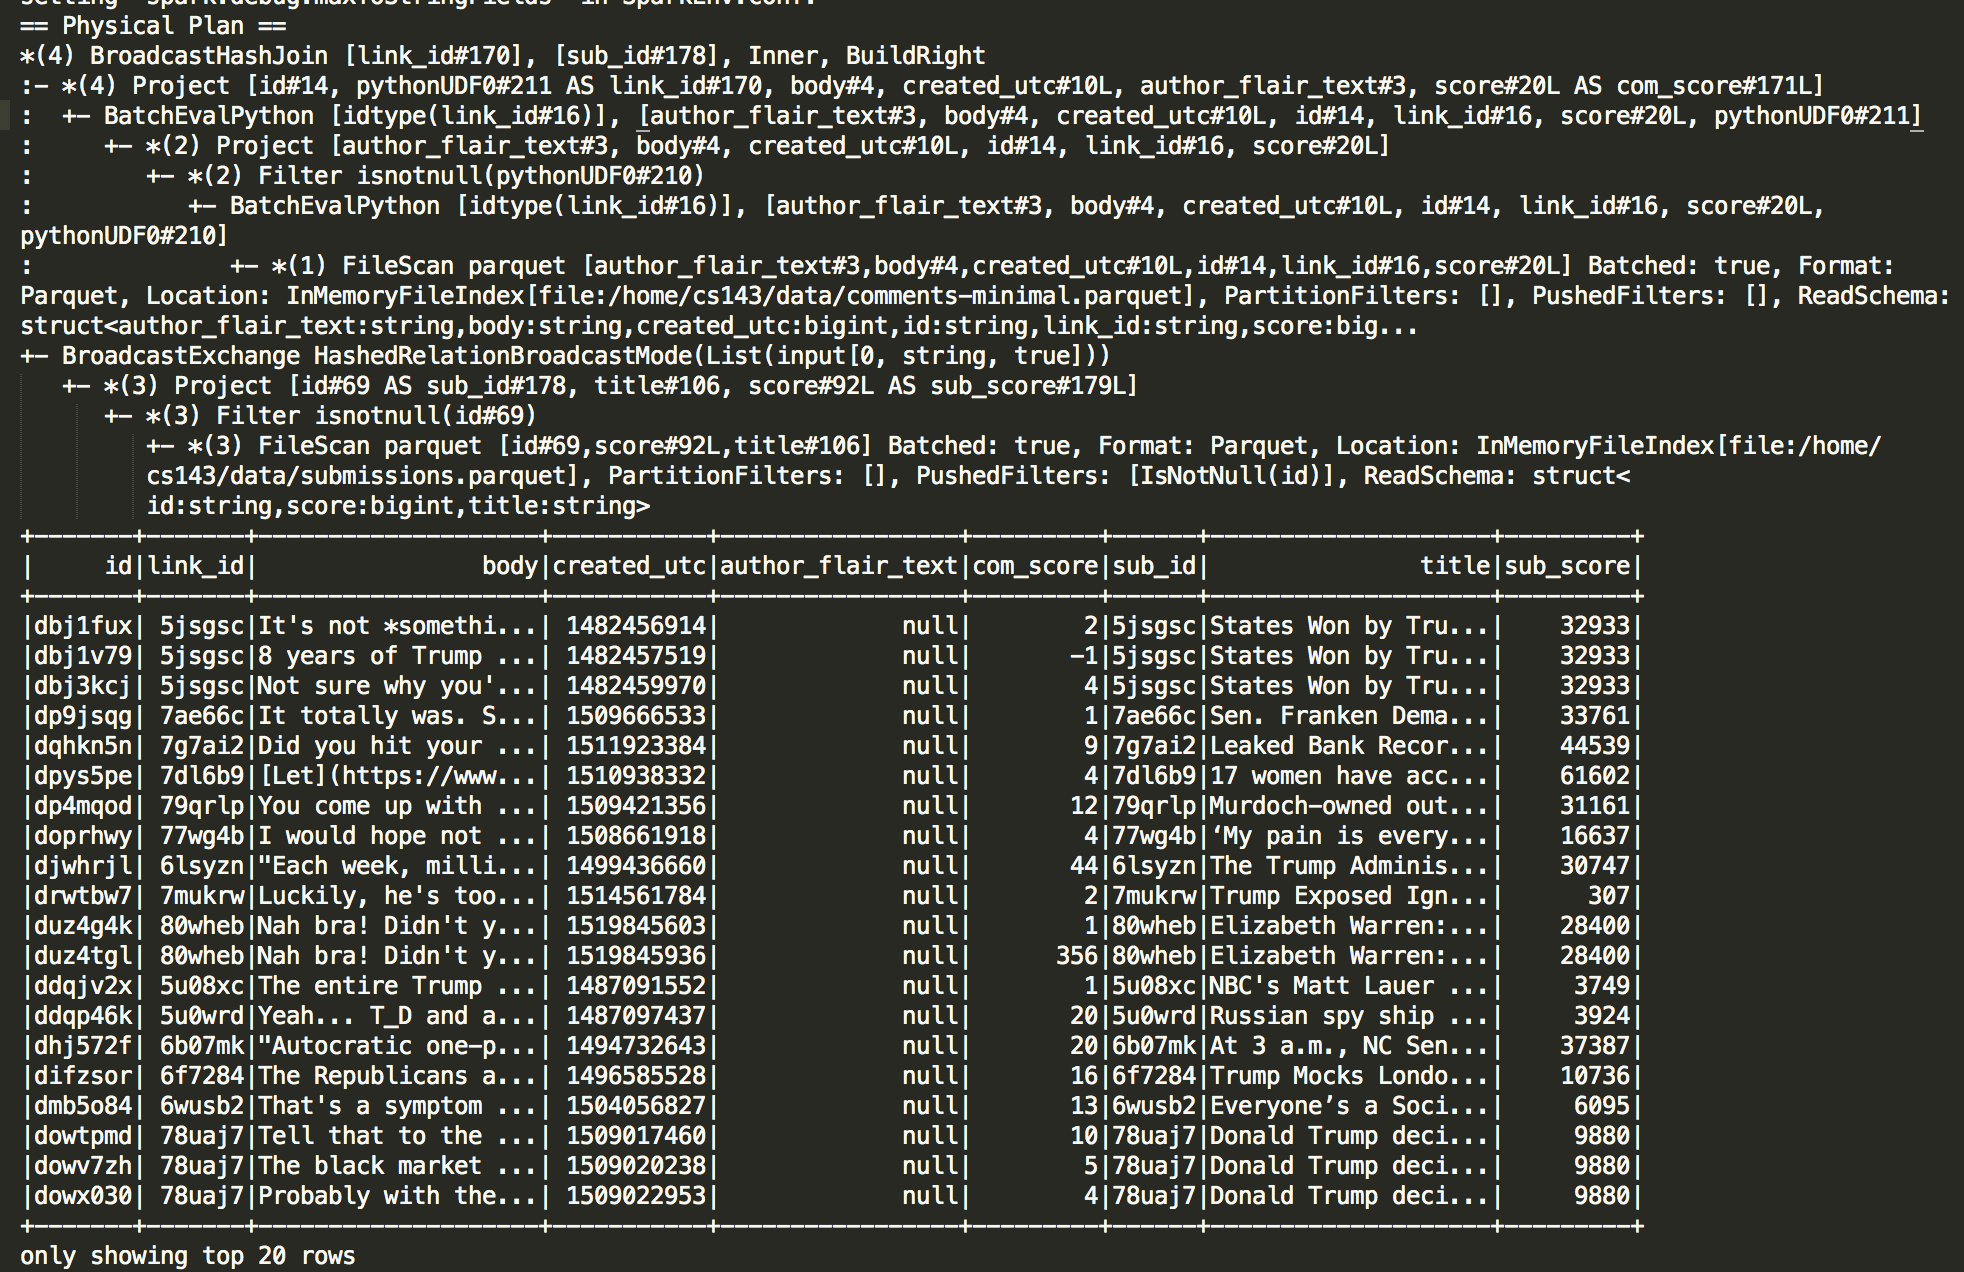
\includegraphics[width=1.12\textwidth]{explain.png}
    \end{center}
    \caption{%
       Explain on Join Operation
     }%sl
     \label {fig:explain}
 \end{figure}
 







\end{document}